\documentclass{article}
\usepackage{graphicx}
\usepackage{authblk}
\usepackage{amsmath}
\usepackage{amsthm}
\usepackage{fancyhdr}
\usepackage[utf8]{inputenc}
\usepackage[margin=1in]{geometry}

\newcommand{\dif}{\mathrm{d}}

\title{\textbf{Dispersion in Electromagnetic Waveguide} \\\vspace{7pt} \small{A Final Project for APPM 4350: Fourier Series and Boundary Value Problems}}
\author[1]{Zach Shelton}
\author[1]{Anna Ikelheimer}
\author[1]{Edward Wawrzynek}
\affil[1]{Department of Electrical, Computer, and Energy Engineering, University of Colorado Boulder}

\date{November 2024}

\pagestyle{fancy}
\lhead{Dispersion in Electromagnetic Waveguide}
\rhead{APPM 4350}

\begin{document}

\maketitle

\section{Introduction}

\section{Waveguide}

% Outline
% 1. Physics (structure & boundary conditions at wall)
% 2. Modes of the waveguide
% 3. Cutoff, propagating vs evanescent modes, phase velocity

\section{Dispersion}

% Outline
% 1. Frequency dependent phase velocity (from previous section)
% 2. Show that the group velocity of envelope of two closely spaced tones differs from their individual phase velocity
% 3. Possible: Treatement of general dispersion across a narrow bandwidth (where B-w curve can be treated as approximately linear) -- via either a superficial qualitative discussion or proper treatment with fourier transform
% 4. Provide an example of the effects of dispersion on a broadband signal (such as a square wave with fundamental just above cutoff)
% (5?). Dispersion under multimode excitation (??????)

% Edward: I'm not sure what the notation we will use in the derivation for waveguide modes is, I can adjust my section to match that before it. The form of the omega-beta relationship will be the same in all cases
In the previous section, we derived the relationship for the phase velocity in the waveguide, 
\begin{equation}\label{eq:waveguide_phase_velocity}
    v_p = \frac{\omega}{\beta} = \frac{c}{\sqrt{1-\frac{\omega_c^2}{\omega^2}}},
\end{equation} which implies \begin{equation}\label{eq:waveguide_dispersion_relation}
    \omega^2(\beta) = c^2\beta^2 + \omega_c^2,
\end{equation} where \(\omega_c\) is the cutoff frequency of the waveguide, \(\omega\) the frequency of operation, and \(\beta\) the phase coefficient.

Notice that \(v_p\) is frequency dependent. This means that the velocity with which a signal propagates down the guide depends on its frequency. Consider a signal containing components at multiple frequencies. The shape of that signal is determined by both the amplitude and phase of those components. If the velocity of these components is not the same, then their relative phases will change as they propagate down the guide, resulting in a received signal which is distorted from the original. A signal which is concentrated will tend to spread out, or disperse, with time. We call this effect dispersion, and we call \eqref{eq:waveguide_dispersion_relation} the dispersion relation for the waveguide.

Not all electromagnetic media are dispersive. The free space, for instance, has a linear dispersion relation of the form \begin{align*}
    \omega^2 = c^2\beta^2, 
\end{align*} which results in a frequency independent phase velocity. Dispersion emerges either from frequency dependence of properties of the system (such as frequency dependent dielectric constant), called material dispersion, or from non-uniform geometries, called geometric dispersion. Dispersion in waveguides is of the geometric type.

\subsection{Group Velocity}

\begin{figure}[h!]
    \centering
    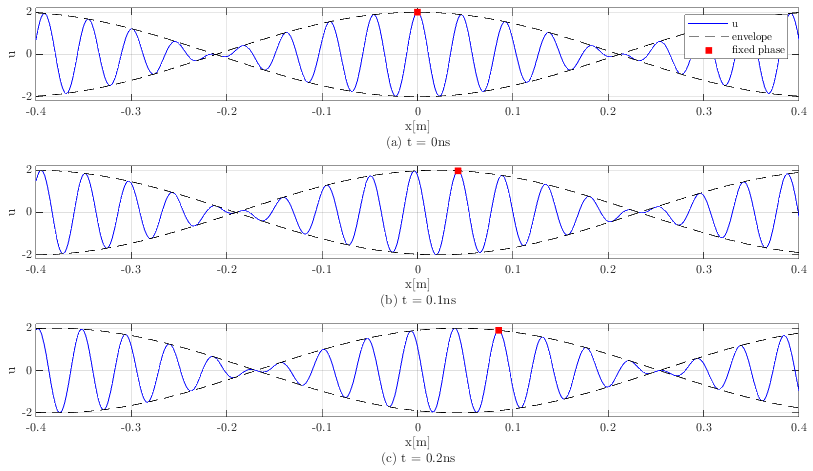
\includegraphics[width=1\textwidth]{figures/dispersion_demo.png}
    \caption{Dispersion of}
    \label{fig:dispersion_demo}
\end{figure}

Equation \eqref{eq:waveguide_phase_velocity} implies that the phase velocity of a frequency above cutoff is greater than the speed of light. Upon first examination, this may seem to contradict physical intuition: we don't expect an electromagnetic wave to propagate faster than light. It turns out that though the phase velocity may be greater than light, the speed of propagation of energy, and therefore also of information, is less than that of light. The speed of energy propagation is described by the group velocity.

% Edward: maybe clarify that \(u\) in this example could represent eg amplitude of TE10 mode. Also maybe use phasors instead of cos (depends what we do before this)
Consider a signal consisting of two harmonic components separated by some small frequency \(\Delta \omega\). The signal consists of an oscillation modulated by a slowly varying envelopse, shown in Figure \ref{fig:dispersion_demo}(a). Due to dispersion, the two components must have different phase coefficients, separated by some small \(\Delta \beta \). As it propagates, the signal is \begin{equation}\label{eq:dispersion_demo_sig}
    u(x, t) = \cos(\beta x - \omega t) + \cos((\beta + \Delta \beta ) x - (\omega + \Delta \omega )t),
\end{equation} where we have from the dispersion relation \eqref{eq:waveguide_dispersion_relation} that \begin{align*}
    \omega^2 &= \omega^2(\beta) = c^2\beta ^2 + \omega _c^2, \\
    (\omega + \Delta \omega )^2 &= \omega^2(\beta + \Delta \beta ) = c^2(\beta + \Delta \beta )^2 + \omega_c^2.
\end{align*} 
Applying the cosine addition rule to \eqref{eq:dispersion_demo_sig}, we have \begin{align*}
    u(x, t) &= 2\cos \left( \frac{\beta  + \beta  + \Delta \beta }{2}x - \frac{\omega + \omega + \Delta \omega }{2}t \right)\cos \left( \frac{\beta  + \Delta \beta - \beta }{2}x - \frac{\omega + \Delta \omega  - \omega}{2}t  \right) \\
    &= 2\cos \left( \left[\beta + \frac{\Delta \beta }{2}\right]x - \left[\omega  + \frac{\Delta \omega }{2}\right]t \right)\cos \left( \frac{\Delta \beta}{2}x - \frac{\Delta \omega}{2}t  \right)
\end{align*} This solution is plotted in Figure \ref{fig:dispersion_demo}. The first cosine term describes the propagation of the carrier of the signal, with velocity \begin{align*}
    v_1 = \frac{2\omega + \Delta \omega }{2\beta + \Delta \beta } \approx \frac{\omega}{\beta } = v_p.
\end{align*} The second cosine describes the propagation of the envelope of the signal, with velocity \begin{align*}
    v_2 = \frac{\Delta \omega }{\Delta \beta }.
\end{align*} As we take \(\beta \to 0\), we call this the group velocity, defined as \begin{align*}
    v_g = \frac{\dif \omega }{\dif \beta }.
\end{align*}
For the waveguide, the group velocity is therefore \begin{equation}\label{eq:waveguide_group_velocity}
    v_g = \frac{\dif \omega }{\dif \beta } = \frac{\dif }{\dif \beta}\left( \sqrt{c^2\beta ^2+\omega_c^2} \right) = \frac{\sqrt{c^2\beta^2+\omega_c^2}}{c^2\beta }.
\end{equation}
We substitute \eqref{eq:waveguide_dispersion_relation} into \eqref{eq:waveguide_group_velocity} and have the group velocity in terms of frequency, \begin{align*}
    v_g = c\sqrt{1 - \frac{\omega_c^2}{\omega^2}}.
\end{align*} For a frequency above cutoff, group velocity is always slower than the speed of light, as expected from physical principles.

% Edward: TODO: actually do plot for above. clarify how group velocity is energy (energy/information contained in envelope, not carrier)

\section{Dispersion in Waveguide}

\section{Measurement}

\end{document}